\section{Results}
\label{sec:results}

We evaluate token pruning across six VLA models spanning three connector families on LIBERO-Object~\cite{liu2023libero} (10 tasks, 50 episodes each, 500 total). All success rates report Wilson 95\% confidence intervals for single-seed results and mean $\pm$ standard deviation for multi-seed results.

\subsection{Taxonomy Overview}
\label{sec:taxonomy_overview}

Table~\ref{tab:taxonomy} organizes seven models into four response classes. The taxonomy reveals that effective vision-to-LLM pipeline complexity, not the nominal connector label or model scale, determines pruning tolerance. Token importance CV tracks this ordering continuously across an 8$\times$ parameter range (450M to 7B): uniformly critical models cluster at CV $< 0.06$, threshold-graded at $\sim$0.15, smooth graded at $\sim$0.22, and catastrophic cliff at $>$0.3. A controlled comparison between $\pi_0$ and OpenVLA (both using 256 SigLIP~\cite{zhai2023siglip} tokens, differing only in connector) yields a 63\,pp gap at $k{=}0.1$, isolating the pipeline as causal (Section~\ref{sec:linear_results}).

The four classes differ qualitatively in their failure mode. Uniformly critical models ($\pi_0$, $\pi_0.5$~\cite{black2025pi05}) distribute importance so evenly that no scoring method can identify dispensable tokens; pruning either preserves random spatial coverage (and survives) or removes a clustered patch (and fails). Threshold-graded models (X-VLA) tolerate removal up to a sharp onset point. Smooth graded models (OpenVLA, OFT, CogACT) degrade proportionally to the fraction removed. Catastrophic cliff models (SmolVLA) collapse at any removal level.

\begin{table*}[t]
\centering
\small
\caption{Seven-model connector taxonomy. CV = coefficient of variation of vision token L2 norms. $^\dagger\pi_0$ reports offline normalized L1 action loss (pending closed-loop evaluation). $^\ddagger$X-VLA uses a linear projection followed by a 12-layer BART encoder; the effective pipeline is not purely linear. $^\S$OFT reports attention entropy and CV only (no pruning evaluation); both metrics match OpenVLA, which confirms the connector determines token importance structure. $^\|$CogACT result from EfficientVLA~\cite{yang2025efficientvla} (literature corroboration, not our evaluation).}
\label{tab:taxonomy}
\begin{tabular}{llcrcll}
\toprule
Model & Connector & Params & Tokens & CV & Representative Result & Class \\
\midrule
$\pi_0$~\cite{black2024pi0} & Linear proj & 3.3B & 256 & 0.038 & $k{=}0.1$: $\mathcal{L}_1{=}0.976$ ($+$2.4\%)$^\dagger$ & Uniformly critical \\
$\pi_0.5$~\cite{black2025pi05} & Linear proj ($\times\!\sqrt{d}$) & 4B & 768 & 0.055 & $k{=}0.5$: L2$=$33.4\%, R$=$69.4\% ($\Delta{=}$+36pp) & Uniformly critical \\
X-VLA~\cite{zheng2025xvla} & Linear proj$^\ddagger$ & 880M & 50 & 0.151 & $k{=}0.9$: $97.8{\pm}0.4$, $k{=}0.85$: $67.8$ & Threshold-graded \\
OpenVLA~\cite{kim2024openvla} & 3-layer MLP & 7B & 256 & 0.215 & $k{=}0.5$: 37.4\% SR ($-$49\%) & Smooth graded \\
OFT~\cite{kim2025openoft} & 3-layer MLP & 7B & 256 & 0.219 & CV $0.219 \approx 0.215$; Ent.\ $0.667 \approx 0.661$$^\S$ & Smooth graded \\
CogACT~\cite{li2024cogact} & MLP proj & -- & -- & -- & 74.2\% SR under 78\% prune$^\|$ & Smooth graded \\
SmolVLA~\cite{shukor2025smolvla} & Pixel-shuffle & 450M & 128 & 0.314 & $k{=}0.95$: 0\% SR & Catastrophic cliff \\
\bottomrule
\end{tabular}
\end{table*}

\subsection{Pixel-Shuffle: Catastrophic Cliff-Edge}
\label{sec:smolvla_results}

The SmolVLA baseline (bypass mode, all 128 vision tokens) achieves 44.8\% SR (224/500, CI [40.5\%, 49.2\%]).\footnote{The official SmolVLA result is 87.3\% SR with batch size 64 on 8 GPUs. Our reproduction uses a smaller batch due to compute constraints.} Every pruning configuration produces 0\% SR across seven configurations varying scoring (learned ACIS vs.\ random), retention ratio ($k \in \{0.50, 0.70, 0.90, 0.95\}$), and mechanism (zero-masking, true removal, token merging). The official SmolVLA checkpoint (59.2\% SR) exhibits identical failure; the cliff-edge is architectural, not a training artifact.

The pattern generalizes across LIBERO suites: Spatial 0.6\%, Goal 0\%. Pixel-shuffle folds each $4{\times}4$ patch block into a single token by channel concatenation; removing one token eliminates an entire $4{\times}4$ receptive field. The resulting spatial entanglement means even 5\% removal ($k{=}0.95$, losing 7 of 128 tokens) destroys task-critical visual information. Full ablation results appear in Table~\ref{tab:smolvla_ablation}, Appendix~\ref{app:smolvla_ablation}.

\subsection{MLP Projector: Smooth Graded Degradation}
\label{sec:openvla_results}

Under random token removal, OpenVLA degrades gracefully across all retention ratios: 74.0\% (baseline) $\rightarrow$ 69.4\% at $k{=}0.95$ ($-4.6$\,pp) $\rightarrow$ 62.0\% at $k{=}0.90$ $\rightarrow$ 49.0\% at $k{=}0.70$ $\rightarrow$ 37.4\% at $k{=}0.50$ $\rightarrow$ 20.6\% at $k{=}0.30$ (Figure~\ref{fig:degradation_curve}; full results with CIs in Table~\ref{tab:openvla_full}, Appendix).\footnote{A second random seed confirms the graded pattern: 62.2\% at $k{=}0.9$ ($+$0.2\,pp), 52.6\% at $k{=}0.7$ ($+$3.6\,pp), 35.6\% at $k{=}0.5$ ($-$1.8\,pp). All within 4\,pp of the primary seed. Per-seed details in Table~\ref{tab:openvla_multiseed}, Appendix~\ref{app:openvla_multiseed}.} At $k{=}0.30$, two tasks reach 0\% SR, but eight retain non-zero performance: degradation is graded, not cliff-edge. Random token removal provides a conservative lower bound on architectural resilience; learned scoring methods would likely yield better retention.

OFT~\cite{kim2025openoft} retains OpenVLA's MLP connector but replaces the action head; its attention entropy (0.667) matches standard OpenVLA (0.661). The connector, not the action head, determines token importance structure. EfficientVLA~\cite{yang2025efficientvla} corroborates the graded pattern from the literature: CogACT~\cite{li2024cogact} (MLP projector) retains 74.2\% SR under 78\% pruning.

To control for scoring method in cross-architecture comparisons, we evaluate L2 norm-based selection on OpenVLA. At moderate-to-aggressive retention ($k \leq 0.7$), L2 performs within 2--4\,pp of random removal (Table~\ref{tab:openvla_l2_vs_random}, Appendix~\ref{app:l2_vs_random}). At $k{=}0.9$, L2 outperforms random by 8.5\,pp (70.6\% vs.\ 62.0\%, reproducible across two random seeds), consistent with the weak but non-zero importance gradient predicted by CV$\,{=}\,$0.215: the signal is exploitable only when few tokens are removed.

\subsection{Linear Projection: From Uniformly Critical to Threshold-Graded}
\label{sec:linear_results}

Three models share a linear projection connector yet exhibit qualitatively different pruning responses. The divergence traces to what happens \emph{after} the projection: nothing ($\pi_0$), a learned scaling ($\pi_0.5$), or a full 12-layer encoder (X-VLA).

\paragraph{$\pi_0$ (3.3B, 256 tokens, pure linear).} Offline normalized L1 action loss at $k{=}0.1$ is 0.976, a 2.4\% \emph{improvement} over the unpruned baseline.\footnote{Offline action loss measures single-step prediction quality; closed-loop evaluation may reveal additional degradation.} CV$\,{=}\,$0.038 indicates near-uniform token norms. Because all tokens carry equal weight, removing 90\% at random preserves spatial coverage and the model compensates.

\paragraph{$\pi_0.5$ (4B, 768 tokens, linear $\times\!\sqrt{d}$).} The baseline achieves 98.2\% SR. This model reveals that low CV does not imply pruning immunity; it implies uniform criticality. The response is strongly method-dependent: random removal at $k{=}0.5$ retains 69.4\% SR ($-$28.8\,pp), while L2 norm-based removal at the same ratio collapses to 33.4\% ($-$64.8\,pp). The gap of 36\,pp is the largest method-dependent effect in our study.

Random removal produces monotonic degradation: 77.2\% at $k{=}0.7$, 69.4\% at $k{=}0.5$, 36.4\% at $k{=}0.3$. L2 norm selection instead produces a V-shaped curve: 55.0\% at $k{=}0.7$, 33.4\% at $k{=}0.5$ (the valley), 51.0\% at $k{=}0.3$. The non-monotonic L2 pattern arises because norm ranking in a low-CV distribution selects spatially clustered tokens (slight norm variations correlate with image regions), and the resulting loss of spatial coverage peaks at intermediate budgets. A second random seed (seed43) confirms the random result: 68.4\% at $k{=}0.5$ ($\Delta{=}$1.0\,pp from seed42).

This result falsifies the ``immune'' assumption from the $\pi_0$ offline evaluation. Low-CV tokens are uniformly critical, not uniformly dispensable. L2 norm-based selection systematically concentrates on spatially correlated tokens and loses coverage; random selection preserves the uniform spatial distribution that these architectures require.

\paragraph{X-VLA (880M, 50 tokens, linear + 12-layer BART).} The 99.2\% baseline is maintained at $k{=}0.95$ ($99.1 \pm 0.2$\%, 3 seeds) and $k{=}0.9$ ($97.8 \pm 0.4$\%) under L2 norm-based removal. A sharp cliff appears at $k{=}0.85$ (67.8\%, $-$30\,pp, 2 seeds), with non-monotonic recovery at $k{=}0.80$ (88.6\%) before degradation resumes: $57.2 \pm 1.6$\% at $k{=}0.7$, $43.4 \pm 0.8$\% at $k{=}0.5$, $22.3 \pm 1.1$\% at $k{=}0.3$, $4.7 \pm 0.6$\% at $k{=}0.2$, and near-zero at $k{=}0.1$. The cliff at $k{=}0.85$ (retaining 42 of 50 BART-encoded tokens) is reproducible across seeds (std $\leq$ 1.6\,pp). The non-monotonic dip is task-specific: four tasks lose $\sim$50\,pp each while six remain unaffected (Table~\ref{tab:xvla_cliff_pertask}, Appendix~\ref{app:xvla_cliff}).

That this threshold appears under importance-based removal (the more favorable test) while OpenVLA degrades smoothly under random removal (the harder test) strengthens the architecture-dependent conclusion. The $\pi_0$--OpenVLA controlled comparison (same 256 SigLIP tokens, same encoder lineage, differing only in connector) produces a 63\,pp gap at $k{=}0.1$, isolating the connector pipeline as the causal factor.

\subsection{VTR: Re-Encoding Overcomes Cliff-Edge}
\label{sec:smart_compress_results}

To test whether learned re-encoding can overcome the pixel-shuffle cliff-edge, we insert a 22.2M-parameter cross-attention module (Vision Token Re-encoder, VTR) between the vision connector and the LLM backbone (details in Appendix~\ref{app:smart_compress_details}). VTR compresses 128 input tokens to $M$ output tokens. Both VTR and the baseline train from the same SmolVLA-Base checkpoint for 100K steps with identical hyperparameters. An extended training control (same procedure without the compressor) achieves 45.0\% SR ($p > 0.9$ vs.\ the 44.8\% baseline); the gain is architectural, not from additional optimization steps.\footnote{The extended baseline also collapses to 0\% SR under pruning ($k{=}0.50$, random, true removal). Additional training does not mitigate the pixel-shuffle vulnerability.}

\begin{table}[t]
\centering
\small
\caption{VTR re-encoding vs.\ deletion on SmolVLA (LIBERO-Object). The M-curve is flat: $M{=}16$ (87.5\% compression) matches $M{=}128$ (no compression) within 1.1\,pp. A parameter-matched MLP adapter achieves comparable SR ($p = 0.15$ vs.\ cross-attention). $^\ddagger$Mean $\pm$ std over 3 seeds (500 episodes each). Other rows: single seed with Wilson 95\% CI.}
\label{tab:smart_compress}
\begin{tabular}{lccrr}
\toprule
Method & $M$ & Red. & SR (\%) & Seeds \\
\midrule
\textit{Baseline} & 128 & 0\% & 44.8 & 1 \\
\textit{Ext.\ training} & -- & -- & 45.0 & 1 \\
\textit{Hard pruning} & -- & 50--90\% & 0.0 & mult. \\
\midrule
Cross-attn$^\ddagger$ & 16 & 87.5\% & 56.9$\pm$1.3 & 55.8/58.4/56.5 \\
Cross-attn$^\ddagger$ & 32 & 75\% & 60.1$\pm$1.3 & 61.6/59.2/59.6 \\
Cross-attn$^\ddagger$ & 64 & 50\% & \textbf{62.0}$\pm$2.3 & 61.6/60.0/64.4 \\
Cross-attn$^\ddagger$ & 96 & 25\% & 54.5$\pm$3.2 & 52.6/58.2/52.8 \\
Cross-attn$^\ddagger$ & 128 & 0\% & 58.0$\pm$3.5 & 59.8/54.0/60.2 \\
MLP adapter$^\ddagger$ & 32 & 75\% & 63.4$\pm$2.6 & 65.2/64.6/60.4 \\
\midrule
\multicolumn{5}{l}{\textit{Official checkpoint (59.2\% baseline)}} \\
Cross-attn & 32 & 75\% & 53.4 & 1 \\
\bottomrule
\end{tabular}
\end{table}

The M-curve is flat (Table~\ref{tab:smart_compress}): $M{=}16$ (56.9\%, 87.5\% compression) performs within 1.1\,pp of $M{=}128$ (58.0\%, no compression), and all five $M$ values cluster within 5\,pp. A parameter-matched MLP adapter (22.14M parameters) achieves 63.4\% $\pm$ 2.6 at $M{=}32$ ($p = 0.15$ vs.\ cross-attention); re-encoding itself, not the attention mechanism, is the operative factor (Figure~\ref{fig:compression_curve}). Cross-suite evaluation confirms generalization: 53.2\% on LIBERO-Spatial and 56.4\% on LIBERO-Goal where hard pruning yields 0\% (Appendix~\ref{app:smart_compress_full}). VTR applied to OpenVLA yields 0\% SR even in passthrough mode ($M{=}128$): it is a targeted remedy for pixel-shuffle entanglement, not a universal compression module.

\subsection{CV Predicts Optimal Pruning Strategy}
\label{sec:scaling_law}

The preceding sections establish that connector architecture determines pruning tolerance. A natural follow-up: can a single diagnostic predict not only \emph{how much} pruning a model tolerates, but also \emph{which} pruning strategy to use? Token importance CV provides exactly this dual prediction. Table~\ref{tab:scaling_law} compares L2 norm-based and random removal at two retention ratios ($k{=}0.5$ and $k{=}0.7$) across three models with measured CV.

\begin{table}[t]
\centering
\small
\caption{L2 norm vs.\ random removal at two retention ratios. The gap $\Delta$(R$-$L2) scales monotonically with CV at both $k{=}0.5$ and $k{=}0.7$: low-CV models require random selection (uniform importance $\rightarrow$ L2 degenerates to spatial clustering), while high-CV models tolerate either strategy. The monotonic ordering holds across retention ratios despite a 2$\times$ change in token budget.}
\label{tab:scaling_law}
\begin{tabular}{lccccc}
\toprule
Model & CV & Tokens & L2 SR (\%) & Random SR (\%) & $\Delta$(R$-$L2) \\
\midrule
\multicolumn{6}{l}{\textit{$k{=}0.5$ (50\% retention)}} \\
$\pi_0.5$ & 0.055 & 768 & 33.4 & \textbf{69.4} & $+$36.0 \\
X-VLA & 0.151 & 50 & 43.4$\pm$0.8 & \textbf{70.3}$\pm$0.9 & $+$26.9 \\
OpenVLA & 0.215 & 256 & 39.2 & 35.8 & $-$3.4 \\
\midrule
\multicolumn{6}{l}{\textit{$k{=}0.7$ (70\% retention)}} \\
$\pi_0.5$ & 0.055 & 768 & 55.0 & \textbf{77.2} & $+$22.2 \\
X-VLA & 0.151 & 50 & 57.2$\pm$1.6 & \textbf{64.2} & $+$7.0 \\
OpenVLA & 0.215 & 256 & \multicolumn{3}{c}{\textit{pending}} \\
\bottomrule
\end{tabular}
\end{table}

The gap decreases monotonically as CV increases at both retention ratios. At $k{=}0.5$: $+$36.0\,pp ($\pi_0.5$, CV$\,{=}\,$0.055) $\rightarrow$ $+$26.9\,pp (X-VLA, CV$\,{=}\,$0.151) $\rightarrow$ $-$3.4\,pp (OpenVLA, CV$\,{=}\,$0.215). At $k{=}0.7$: $+$22.2\,pp $\rightarrow$ $+$7.0\,pp $\rightarrow$ pending. The monotonic ordering holds across a 2$\times$ change in absolute token budget, strengthening the claim that CV captures a structural property of the connector rather than a coincidence at a single operating point.

The mechanism is intuitive. When tokens have near-uniform L2 norms (low CV), norm ranking captures spatial artifacts rather than genuine importance differences. L2 norm-based selection then clusters on correlated patches and loses spatial coverage, while random selection preserves the uniform distribution these models depend on. As CV rises, a genuine importance gradient emerges that L2 norm ranking can exploit; the random-vs-L2 advantage vanishes and eventually reverses.

CV therefore serves as a dual predictor. First, it predicts tolerance class: low CV signals uniform criticality (sensitive to method choice but potentially robust under the right strategy), moderate CV signals a threshold or graded response, and high CV signals extreme fragility (catastrophic cliff). Second, it predicts optimal strategy: models below CV $\approx 0.15$ should use coverage-preserving methods (random or spatially uniform selection), while models above this threshold can benefit from importance-based scoring.

At extreme compression ($k{=}0.3$), the interaction partially reverses for $\pi_0.5$: L2 norm achieves 51.0\% vs.\ random 36.4\% ($\Delta{=}-$14.6\,pp favoring L2). The optimal strategy also depends on the absolute token budget; when very few tokens remain, even spatially clustered high-norm tokens provide more signal than a sparse random sample. Full analysis of this interaction appears in Appendix~\ref{app:cv_strategy_interaction}.

\begin{figure}[t]
\centering
\begin{subfigure}[b]{0.48\linewidth}
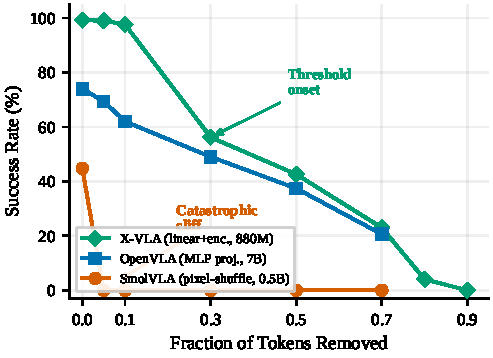
\includegraphics[width=\linewidth]{figures/paper/fig_degradation_curve.pdf}
\caption{Token pruning across connector classes.}
\label{fig:degradation_curve}
\end{subfigure}
\hfill
\begin{subfigure}[b]{0.48\linewidth}
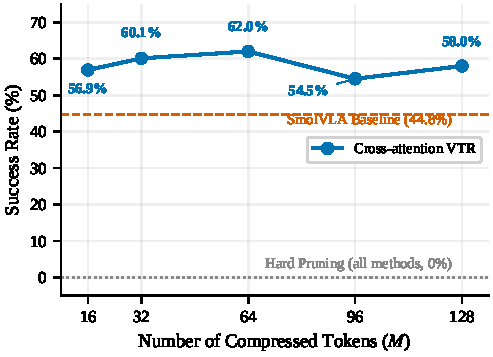
\includegraphics[width=\linewidth]{figures/paper/fig_compression_curve.pdf}
\caption{VTR M-curve and CV-strategy interaction.}
\label{fig:compression_curve}
\end{subfigure}
\caption{Architecture-dependent response to token reduction on LIBERO-Object. (a)~Pruning across pipeline types: pure linear ($\pi_0$) is uniformly critical, linear+encoder (X-VLA) is threshold-graded (onset at $k{=}0.85$), MLP (OpenVLA) degrades smoothly, pixel-shuffle (SmolVLA) collapses. (b)~VTR re-encoding achieves near-lossless compression ($M{=}16 \approx M{=}128$) where deletion yields 0\%; CV predicts the L2-vs-random gap monotonically.}
\label{fig:results_combined}
\end{figure}
